\documentclass[11pt]{article}
    
\usepackage{amsmath}
\usepackage{amsfonts}
\usepackage{cite}
\usepackage[letterpaper, total={6.5in, 9in}]{geometry}
\usepackage{mathpazo}
\usepackage{sourcecodepro}
\usepackage{graphicx}
\usepackage[dvipsnames]{xcolor}
\usepackage{hyperref}
  \hypersetup{
    colorlinks=true,
    allcolors=MidnightBlue,
    pdftitle={Efficient unconstraining parameter transforms for Hamiltonian Monte Carlo},
    pdfpagemode=FullScreen
  }
\usepackage[title]{appendix}

\newcommand{\setcomp}[2]{\left\{ #1 \ \Big|\ #2 \right\}}
\newcommand{\rngto}[1]{1{:}#1}
\newcommand{\abs}[1]{\left| #1 \right|}
\newcommand{\absdet}[1]{\abs{#1}}
\newcommand{\dv}[1]{\mathrm{d}{#1}}
\newcommand{\Exp}{\mathrm{Exp}}
\newcommand{\vect}{\mathrm{vec}}
\newcommand{\vectu}{\mathrm{vecu}}

\begin{document}


\title{Efficient Simplex Parameterizations for Hamiltonian Monte Carlo}
\author{Meenal Jhajharia
        \\ \small Center for Computational Mathematics
        \\ \small Flatiron Institute
\and \large Seth D. Axen
     \\ \small Cluster of Excellence Machine Learning
     \\ \small New Perspectives for Science
     \\ \small University of T\"ubingen
\and Adam Haber
     \\ \small Weizmann Institute of Science
\and Sean Pinkney
     \\ \small Center of Excellence
     \\ \small Omnicom Media Group
\and Bob Carpenter
     \\ \small Center for Computational Mathematics
     \\ \small Flatiron Institute
}
\date{DRAFT: \today}
\maketitle

\begin{abstract}
  \noindent
  We consider the task of sampling on a unit $N$ - Simplex using Hamiltonian Monte Carlo. In bayesian computation, parameters are often constrained on a simplex, e.g. for modelling categorical data. Unconstraining transforms mapping a unit $N$ - Simplex to $R^N$ are used to avoid the challenges of constructing HMC samplers for a constrained space. Arbitrary transformations can serve as this mapping, not all of them work well when sampled from - owing to weak convexity, incompatible posterior geometry, numerical instability among other reasons. In this paper we evaluate the statistical properties,  computational efficiency and geometry for unconstraining transforms between a unit $N$ - simplex and $R^N$.
  
  \end{abstract}

\section{Introduction}

In statistical computing, we often need to compute high-dimensional integrals over densities $\pi(x)$ (e.g., Bayesian estimation or prediction, $p$-value calculations, etc.).  The only black-box techniques that work for general high-dimensional integrals are Markov chain Monte Carlo (MCMC) methods.  The most effective MCMC method in high dimensions is Hamiltonian Monte Carlo (HMC) \cite{neal2011mcmc}. HMC works by simulating the Hamiltonian dynamics of a fictitious particle representing the value being sampled coupled with a momentum term. 

Although it is possible to construct HMC samplers that work for simple constraints such as upper- and/or lower-bounds \cite{neal2011mcmc} or unit vectors \cite{byrne2013geodesic}, it is much more challenging to do the same for complex constraints such as simplexes, positive definite matrices or for densities involving multiple constrained values.  Instead, it is far more common to map the constrained values to unconstrained values before sampling \cite{JSSv076i01, radul2021base, fjelde2020bijectors}.

This approach is not without ramifications, posterior geometry obtained from a transformed variable can be very different from the original. In context of Hamiltonian Monte Carlo, there is a lack of formal analysis or comparison for these transformations.  We evaluate both standard and relatively unvisited transforms for constrained data types that find regular use in statistical modeling. Evaluation takes into account specificities such as head, body, and tail of distributions in terms of computational efficiency of the transform, its Jacobian determinant and associated gradients, the geometry induced in the unconstrained space (e.g., log convexity and conditioning), as well as HMC sampling efficiency.

In this paper, we focus on transforms on a unit $N$-simplex. Simplexes are useful for representations of multinomial probabilities - points on the standard $N$-simplex in $R^{N+1}$ are the space of possible parameters (probabilities) of the categorical distribution on $n+1$ possible outcomes. Lastly, we define Aitchison Geometry and compare metric distortions of canonical transforms (or their augmented forms) in Compositional Data Analysis.
\section{Constraining transforms}

A surjective constraining transform $f : \mathcal{Y} \rightarrow \mathcal{X}$ is mapped from an unconstrained space $\mathcal{Y} = \mathbb{R}^M$ onto a constrained space $\mathcal{X} \subset \mathbb{R}^N$, and $h(y)$ is a proper density defined over $y \in \mathcal{Y}$ such that if $y \sim h(\cdot)$, then $f(y) \sim \textrm{uniform}(\cdot \mid \mathcal{X})$.  It is not possible to sample over an improper density.  To this end, we stipulate the induced distribution on $y$ to be proper, given a proper density $p_X(x)$ defined for $x \in \mathcal{X}$ such that if $y \sim p_Y(\cdot)$ then $f(y) \sim p_X(\cdot)$ . In this case, density of the distribution induced on $y$ is 
\[
p_Y(y) = h(y) \, p_X(f(y))
\]

\subsection{Bijective constraining transforms}

 Suppose, we have a distribution $p_X(x)$ on constrained values $x \in \mathcal{X}$. A smooth, bijective unconstraining transform is defined as $g : \mathcal{X} \rightarrow \mathcal{Y}$, and $g^{-1}$ is the constraining transform $f : \mathcal{Y} \rightarrow \mathcal{X}$.  Using the standard change of variables, the induced density on $\mathcal{Y}$ is adjusted by a constant factor 
 
 \[\absdet{J_f(y)} = \absdet{\nabla_y \, f(y)}.
 \]
Thereby, for any given $p_X(x)$, 
 
 \[
 y \sim p_Y(\cdot) \implies f(y) \sim p_X(\cdot) \, \, \text{where} \, \, p_Y(y) = p_X(f(y)) \, \absdet{J_f(y)}
\]


\subsection{Surjective constraining transforms}


For a constraining transform $f: R^\mathcal{M} \rightarrow R^\mathcal{N}$, if $\mathcal{M} >  \mathcal{N}$, additional constraints are needed to ensure the correct distributions on $\mathcal{X}$. Bijective change-of-variables method cannot be applied here, instead an expanded parameter space $\mathcal{Z} = \mathcal{X} \times \mathcal{R}$ is constructed with parameters $z = (x, r)$. Here, $r \in \mathcal{R}$ is introduced such that $\mathcal{Y}$ and $\mathcal{Z}$ have the same dimensionality. Taking prior $p_R(r | x)$,
\[
p_Y(y) = h(y) p_Z(z) = h(y) p_X(x) p_R(r | x).
\]
We define a bijective transform $\tilde{g}: \mathcal{Z} \to \mathcal{Y}$ and its inverse $\tilde{f}$, where $\tilde{f}(y)_1 = f(y)$, this permits obtaining change-of-variables,
\[
h(y) = |J_{\tilde{f}}(y)|.
\]
Discarding $r$ after sampling is equivalent to marginalizing it out, and in practice, $r$ may never be directly computed. On acount of convenience,  we choose $p_R(r | x) = p_R(r)$ in the rest of the paper.

% In all of these cases, we will have a $p_Y(y)$ defined as a product of the change-of-variables adjustment for the transform coupled with a standard normal distribution over $\mathcal{Y}$,
% \[
%   h(y) = \textrm{normal}(y \mid 0, \textrm{I}) \, \absdet{J_f(y)},
% \]  
% where $\textrm{I}$ is the identity matrix.
% For each case, we have to ensure that $p_Y(y) = h(y) \, p_X(f(y))$ is such that if $y \sim p_Y(\cdot)$, then $f(y) \sim p_X(\cdot)$.

\section{Unit simplex}

The set of unit simplexes of dimension $N$ is
\[
  \Delta^N = \setcomp{x \in \mathbb{R}^{N + 1}}{\sum_{i=1}^{N + 1} x_i = 1,\,x_i \ge 0 \, \, \forall i }
\]
An affine transformation $(x_0, \ldots, x_n) \mapsto \sum_{i=0}^n x_i v_i \,$ maps a unit $N$-simplex to an arbitrary $N$-simplex. Geometrically, $\Delta^N$ is the convex hull of $N+1$ standard unit vectors comprising the vertices.  For example, $\Delta^2$ is the convex closure of the three vectors
$\begin{bmatrix}1 & 0 & 0 \end{bmatrix},
\begin{bmatrix} 0 & 1 & 0 \end{bmatrix}$,
and $\begin{bmatrix} 0 & 0 & 1 \end{bmatrix}$. As such, there are only $N$ degrees of
freedom, because if $x$ is an $N$-simplex, then
\[
  x_{N+1} = 1 - (x_1 + x_2 + \cdots + x_N).
\]
We introduce the notation $\Delta^N_-$ to denote the probability simplex, which is a face of the unit simplex (each face of an $N$ - simplex is an affine $N-1$ - simplex),

\[
\Delta^N_-
= 
\setcomp{x \in \mathbb{R}^N}{x_n \geq 0 \textrm{ for } 1 \leq n \leq N \textrm{ and } \sum_{n=1}^N x_n \leq 1}.
\]
There is a bijective mapping between $\Delta^N_-$ and $\Delta^N$ defined for $x \in \Delta^N_-$ by 
\[
f(x) = \begin{bmatrix} x_1 & x_2 & \cdots x_N & 1 - \sum_{n=1}^N x_n \end{bmatrix}.
\]

\subsection{Aitchison Geometry}

Compositional data analysis deals with vectors of strictly positive quantities that adhere to a constant sum constraint. \cite{aitchison1982statistical} defined compositional data on a simplical space:
$$
\Delta^N=\left\{\mathbf{x}=\left[x_1, x_2, \ldots, x_D\right] \in \mathbb{R}^N \mid x_i>0, i=1,2, \ldots, N ; \sum_{i=1}^N x_i=\kappa\right\}
$$

Relative information enclosed in compositional data is preserved under non-negative scalar multiplication, thus we often consider $\mathcal{S}^D$ to be a standard simplex, where the constant $\kappa$ is 1. This can be achieved by normalization, defined by a closure operator in Aitchison Geometry as follows:
$$
\mathcal{C}\left[x_1, x_2, \ldots, x_N\right]=\left[\frac{x_1}{\sum_{i=1}^N x_i}, \frac{x_2}{\sum_{i=1}^N x_i}, \ldots, \frac{x_N}{\sum_{i=1}^N x_i}\right].
$$

Aitchison defines three linear isomorphisms on this simplex - Additive Log Ratio, Centered Log Ratio and Isometric Log Ratio. In the rest of the paper, we discuss transforms on the simplex - including these three classical ones or augmented forms of them that are bijective.


\subsubsection{Additive log ratio transform}
The unconstraining transform for the identified softmax is known as
the additive log ratio (ALR) transform
\cite{aitchison1982statistical}, which is a bijection
$\textrm{alr}:\Delta^{N-1} \rightarrow \mathbb{R}^{N-1}$ defined for
$x \in \Delta^{N-1}$ by
\[
  \textrm{alr}(x)
  = \begin{bmatrix}\displaystyle
    \log \frac{x_1}{x_N}, \cdots , \log \frac{x_{N-1}}{x_N}
  \end{bmatrix}
\]
The inverse additive log ratio transform maps values in
$\mathbb{R}^{N-1}$ to $\Delta^{N-1}$ defined for $y \in
\mathbb{R}^{N-1}$ by
\[
  \textrm{alr}^{-1}(y)
  = \textrm{softmax}(\begin{bmatrix} y &  0 \end{bmatrix}),
\]
where for $u \in \mathbb{R}^N$,

\[
  \textrm{softmax}(u) = \frac{\exp(u)}{\sum \exp(u)}
\]

\[
\textrm{Here, } \abs{J} = \prod \exp(y)
  \, \left( \frac{1}{1 + \sum(\exp(y))} \right)^N
\]

Geometrically, coordinates obtained from an Additive Log Ratio transform do not correspond to an orthogonal basis, rather it is an oblique basis with respect to the Aitchison metric. Also, the transform is not symmetrical in all the N components, rather only the first N-1. This distorts euclidean distances measured from the ALR coordinates
\subsubsection{Stick-Breaking Transform}

The stick-breaking transform is derived from the standard construction for Dirichlet processes \cite{sethuraman1994constructive}. The inverse mapping from unconstrained to constrained parameters involves taking a unit-length stick and recursively breaking pieces off until it is divided into $N + 1$ pieces, the lengths of which provide the entries in the simplex.  Following the transforms used by Stan \cite{stan2022ref}, we add an offset so that the unconstraining transform of the uniform simplex $x = \begin{bmatrix} 1/N & \cdots & 1/N \end{bmatrix}$ maps to $y = \begin{bmatrix} 0 & \cdots & 0 \end{bmatrix}$, a vector of zeros.

\paragraph{Unconstraining transform}
The unconstraining transform $f : \Delta^{N} \to  \mathbb{R}^N$ is defined so that if $f(x) = y$, then
\[
y_n
= \mathrm{logit}(z_n)
  - \mbox{log}\left(\frac{1}{N + 1 - n} \right),
\]
where 
\[ 
 z_n = \frac{x_i}{1 - \sum_{i = 1}^{n-1} x_{i}}.
\]

\paragraph{Constraining inverse transform}
The inverse transform follows the stick breaking construction, with $f^{-1} \colon \mathbb{R}^N \to \Delta^N$ defined by $f^{-1}(y) = x$, where
\[
x_n = z_n \left( 1 - \sum_{i=1}^{n-1} x_i \right), \\
\]
with
\[
z_n = \mathrm{logit}^{-1}\!\left(
y_n  + \log \left( \frac{1}{N - n} \right)
\right).
\]
                                            
\paragraph{Change-of-variables adjustment} 
The absolute determinant of the Jacobian of the inverse transform is
\[
\abs{J_{f^{-1}}} 
= \prod_{n=1}^{N-1}
   z_n \, (1 - z_n)
   \left( 1 - \sum_{i=1}^{n-1} x_{i} \right).
\]

% \subsubsection{Additive log ratio transform}
% The unconstraining transform for the identified softmax is known as
% the additive log ratio (ALR) transform
% \cite{aitchison1982statistical}, which is a bijection
% $\textrm{alr}:\Delta^{N-1} \rightarrow \mathbb{R}^{N-1}$ defined for
% $x \in \Delta^{N-1}$ by
% \[
%   \textrm{alr}(x)
%   = \begin{bmatrix}\displaystyle
%     \log \frac{x_1}{x_N}, \cdots , \log \frac{x_{N-1}}{x_N}
%   \end{bmatrix}
% \]
% The inverse additive log ratio transform maps values in
% $\mathbb{R}^{N-1}$ to $\Delta^{N-1}$ defined for $y \in
% \mathbb{R}^{N-1}$ by
% \[
%   \textrm{alr}^{-1}(y)
%   = \textrm{softmax}(\begin{bmatrix} y &  0 \end{bmatrix}),
% \]
% where for $u \in \mathbb{R}^N$,

% \[
%   \textrm{softmax}(u) = \frac{\exp(u)}{\sum \exp(u)}
% \]

% \[
% \textrm{Here, } \abs{J} = \prod \exp(y)
%   \, \left( \frac{1}{1 + \sum(\exp(y))} \right)^N
% \]

\subsubsection{Isometric Log Ratio Transform}

We may define a distance preserving transformation from $\textrm{ilr}:\Delta^{N-1} \rightarrow \mathbb{R}^{N-1}$ called an isometric log ratio transform. By noting that the ALR transformation may be written as

\[
  \begin{aligned}
 \textrm{alr}(x) &= \begin{bmatrix}\displaystyle
    \log \frac{x_1}{x_N} \cdots \log \frac{x_{N-1}}{x_N}
  \end{bmatrix} \\
  &= \log(\mathbf{x}) \cdot \begin{bmatrix}\displaystyle
                    1 & 0 & \cdots & 0 \\
                    0 & 1 & \cdots & 0 \\
                    \vdots & \vdots & \ddots & \vdots \\
                    0 & 0 & \cdots & 1 \\
                    -1 & -1 & \cdots & -1
                    \end{bmatrix}.
  \end{aligned}
\]
Take any unitary matrix $\mathbf{V} \in D \times D - 1$ then the ILR is defined for $x \in \Delta^{N-1}$ by
\[
  \textrm{ilr}(x)
  = \log(\mathbf{x}) \cdot \mathbf{V}.
\]

Unitary $\mathbf{V}$ matrices may be constructed through the Gram-Schmidt process or by normalizing the rows of a Helmert contrast matrix using the L2 norm.

The inverse isometric log ratio transform maps values in
$\mathbb{R}^{N-1}$ to $\Delta^{N-1}$ defined for $y \in
\mathbb{R}^{N-1}$ by
\[
  \textrm{ilr}^{-1}(y)
  = \textrm{softmax}(\begin{bmatrix} \exp(\mathbf{V^{-1}} \mathbf{x} ) \end{bmatrix}),
\]
where for $u \in \mathbb{R}^N$,
\[
  \textrm{softmax}(u) = \frac{\exp(u)}{\textrm{sum}(\exp(u))}.
\]

The affine transformation of the multiplication by the inverse unitary matrix does not change
the calculation of the change of variables adjustment proceeds similarly to the ALR case. In fact, any affine transformation may be completed at this stage which generalizes the ILR to power transformations as in \cite{tsagris2011data}\footnote{
   Let $\alpha$ be the scalar power transformation parameter in $\mathbb{R}$ then the inverse \textit{power} based transformation is given by $(V^{-1} \mathbf{x} \alpha + 1) / \alpha$. See \cite{tsagris2011data} for more information.
}. 

Given a density $p_X(x)$ defined over simplices $x \in \Delta^{N-1}$,
we can transform to a density over unconstrained parameters $y \in
\mathbb{R}^{N-1}$ by applying the inverse ILR transform and adjusting
for the change of variables, which yields
\[
  p_Y(y) = p_X(\textrm{ilr}^{-1}(y)) \absdet{J_{s}(y)},
\]
where $J_{s}(y)$ is the Jacobian of the function $s$ evaluated at $y$
and $\absdet{J_s(y)}$ is the absolute value of its determinant.

\subsubsection{Augmented-Softmax Transform}
%TODO:  Needs to be written like other transforms -> transform, inverse, |J|
We define the constraining transformation
$f: \mathbb{R}^N \to \Delta^{N} \times \mathbb{R}_{>0}: y \mapsto
(x_-, r)$, where and $x_{-} \in \Delta_{-}^N$. Here $r = \sum_{i=1}^N \textrm{exp}(y_i) > 0$,
$x_i = \frac{1}{r} \textrm{exp}(y_i)$ for $i \in [1, N-1]$ and $\delta_{ij}$ is the Kronecker delta function. If $\mathrm{diag}(x)_{i, j} = \delta_{ij} x_i$ and $\boldsymbol{1}_n$ is the $N$-vector of ones, then
\[
  J_f = (I_{N-1} - x_- \boldsymbol{1}_{N-1}^\top) \operatorname{diag}(x_-),
\] 

Using Sylvester's determinant theorem,
$|I_{N-1} - x_- \boldsymbol{1}_{N-1}^\top| = 1 -
\boldsymbol{1}_{N-1}^\top x_- = 1 - \sum_{i=1}^{N-1} x_i = x_N$, so
$$ |J_f| = x_n \prod_{i=1}^{N-1} x_i = \prod_{i=1}^{N} x_i = \exp\left(\sum_{i=1}^{N-1} y_i\right) \left(1 + \sum_{i=1}^{N-1} \exp(y_i)\right)^{-N}$$

\subsubsection{Hyperspherical coordinate transforms}

Let $u$ be a unit vector with $N+1$ elements in the positive orthant of the unit sphere $\mathbb{S}_{>0}^N$, which has the constraints $\sum_{i=1}^{N+1} u_i^2 = 1$ and $u_i > 0$.
There is a unique bijective map $f_1\colon \mathbb{S}_{>0}^N \to \Delta^N \colon u \mapsto x$ given by $x_i = u_i^2$.
We then define $f_2$ as the map from hyperspherical coordinates to Cartesian coordinates of the hypersphere.
Taking $z_i = \sin^2(\phi_i) \in (0, 1]$ for $\phi_i \in (0, \frac{\pi}{2}]$, the composed map $f_1 \circ f_2$ is written

\[
  x_i = (1 - z_i (1 - \delta_{i,N+1})) \prod_{k=1}^{i-1} z_k.
\]

The inverse of this transform is
$$z_i = 1 - \frac{x_i}{1 - \sum_{k=1}^{i - 1} x_k}.$$

To complete the transform $f = f_1 \circ f_2 \circ f_3$, we must select a constraining transform $f_3: y \mapsto \phi$.
We consider 3 different approaches.

\subsubsection{Hyperspherical angular transform}

Here we use a (scaled) logistic function to map directly from the unconstrained space to the constrained angle:
$$\sin^{-1}(\sqrt{z_i}) = \phi_i = \frac{\pi}{2} \operatorname{logit}^{-1} (y_i).$$

In terms of $\phi$,

$$
|J_f| = 2^N \prod_{i=1}^N \phi_i \left(1 - \frac{2}{\pi} \phi_i\right) \sin^{2(N-i)+1}(\phi_i) \cos(\phi_i).
$$
This transform was discussed in \cite{betancourt2012cruising}.

\subsubsection{Hyperspherical logit transform}

If we define $f_3$ to map from the unconstrained space directly to a conveniently-chosen power of $z_i$ function using the logistic function 
$$z_i^{N-i+1} = \operatorname{logit}^{-1} (y_i),$$
then the Jacobian determinant is
$$
|J_f| = \frac{1}{N!} \prod_{i=1}^N \operatorname{logit}^{-1}(y_i) (1 - \operatorname{logit}^{-1}(y_i)).
$$
If $x$ is uniformly distributed on the unit simplex, then $y_i$ is logistic-distributed with mean 0 and variance $\frac{\pi^2}{3}$.

\subsubsection{Hyperspherical probit transform}

Similarly, if we use the inverse probit function instead of the inverse logit, then $f_3$ is
$$z_i^{N-i+1} = \operatorname{probit}^{-1} (y_i),$$
where $\operatorname{probit}^{-1}(\cdot)$ is the cumulative distribution function of the standard normal distribution.
The resulting Jacobian determinant is
\[
|J_f| = \frac{1}{N!} \prod_{i=1}^N \mathcal{N}(y_i),
\]
where $\mathcal{N}(\cdot)$ is the density function of the standard normal distribution.
As a result, if $x$ is uniformly distributed on the unit simplex, then $y_i$ is standard normally distributed.

%TODO: better captions
\section{Results}

\begin{table}[!ht]
    \centering
    \begin{tabular}{r|r|r|r|r|r|}
    \hline
        $\alpha$ & $N$ & Stan & Augmented-Softmax & softmax & stickbreaking \\ \hline
        0.1 & 10  & 6.9s & 11.712s & 10.548s & 13.386s \\ 
        0.1 & 100 & 74.274s & 33.757s & 61.826s & 159.016s \\ 
        0.1 & 1000 & 1108.48s & 307.463s & 657.791s & 11773.4s \\ 
        1 & 10 & 4.072s & 6.328s & 5.337s & 5.67s \\ 
        1 & 100 & 20.805s & 27.151s & 25.94s & 51.45s \\ 
        1, & 1000 & 306.942s & 171.824s & 184.126 & 3023.24 \\ 
        10 & 10 & 4.123s & 6.375s & 5.563s & 5.606s \\ 
        10 & 100 & 23.6s & 29.091s & 30.747s & 48.834s \\ 
        10 & 1000 & 205s.627 & 161.11s & 150.751s & 1866.83s \\ \hline
    \end{tabular}
\end{table}

\begin{table}[!ht]
    \centering
    \begin{tabular}{c|r||r|r|r|r|}
        $\alpha$ & $N$ & stan & aug-softmax & softmax & stick-break \\ \hline 
        0.1 & 10  & 7s & 11s & 11s & 13s \\ 
        0.1 & 100 & 74s & 34s & 62s & 160s \\ 
        0.1 & 1000 & 1100s & 300s & 660s & 12000s \\ 
        1 & 10 & 4s & 6s & 5s & 6s \\ 
        1 & 100 & 21s & 27s & 26s & 51s \\ 
        1 & 1000 & 300s & 170s & 180s & 3000s \\ 
        10 & 10 & 4s & 6s & 6s & 5s \\ 
        10 & 100 & 24s & 29s & 31s & 49s \\ 
        10 & 1000 & 200s & 160s & 150s & 1900s \\
    \end{tabular}
\end{table}

\begin{figure}[t!]
    \centering
    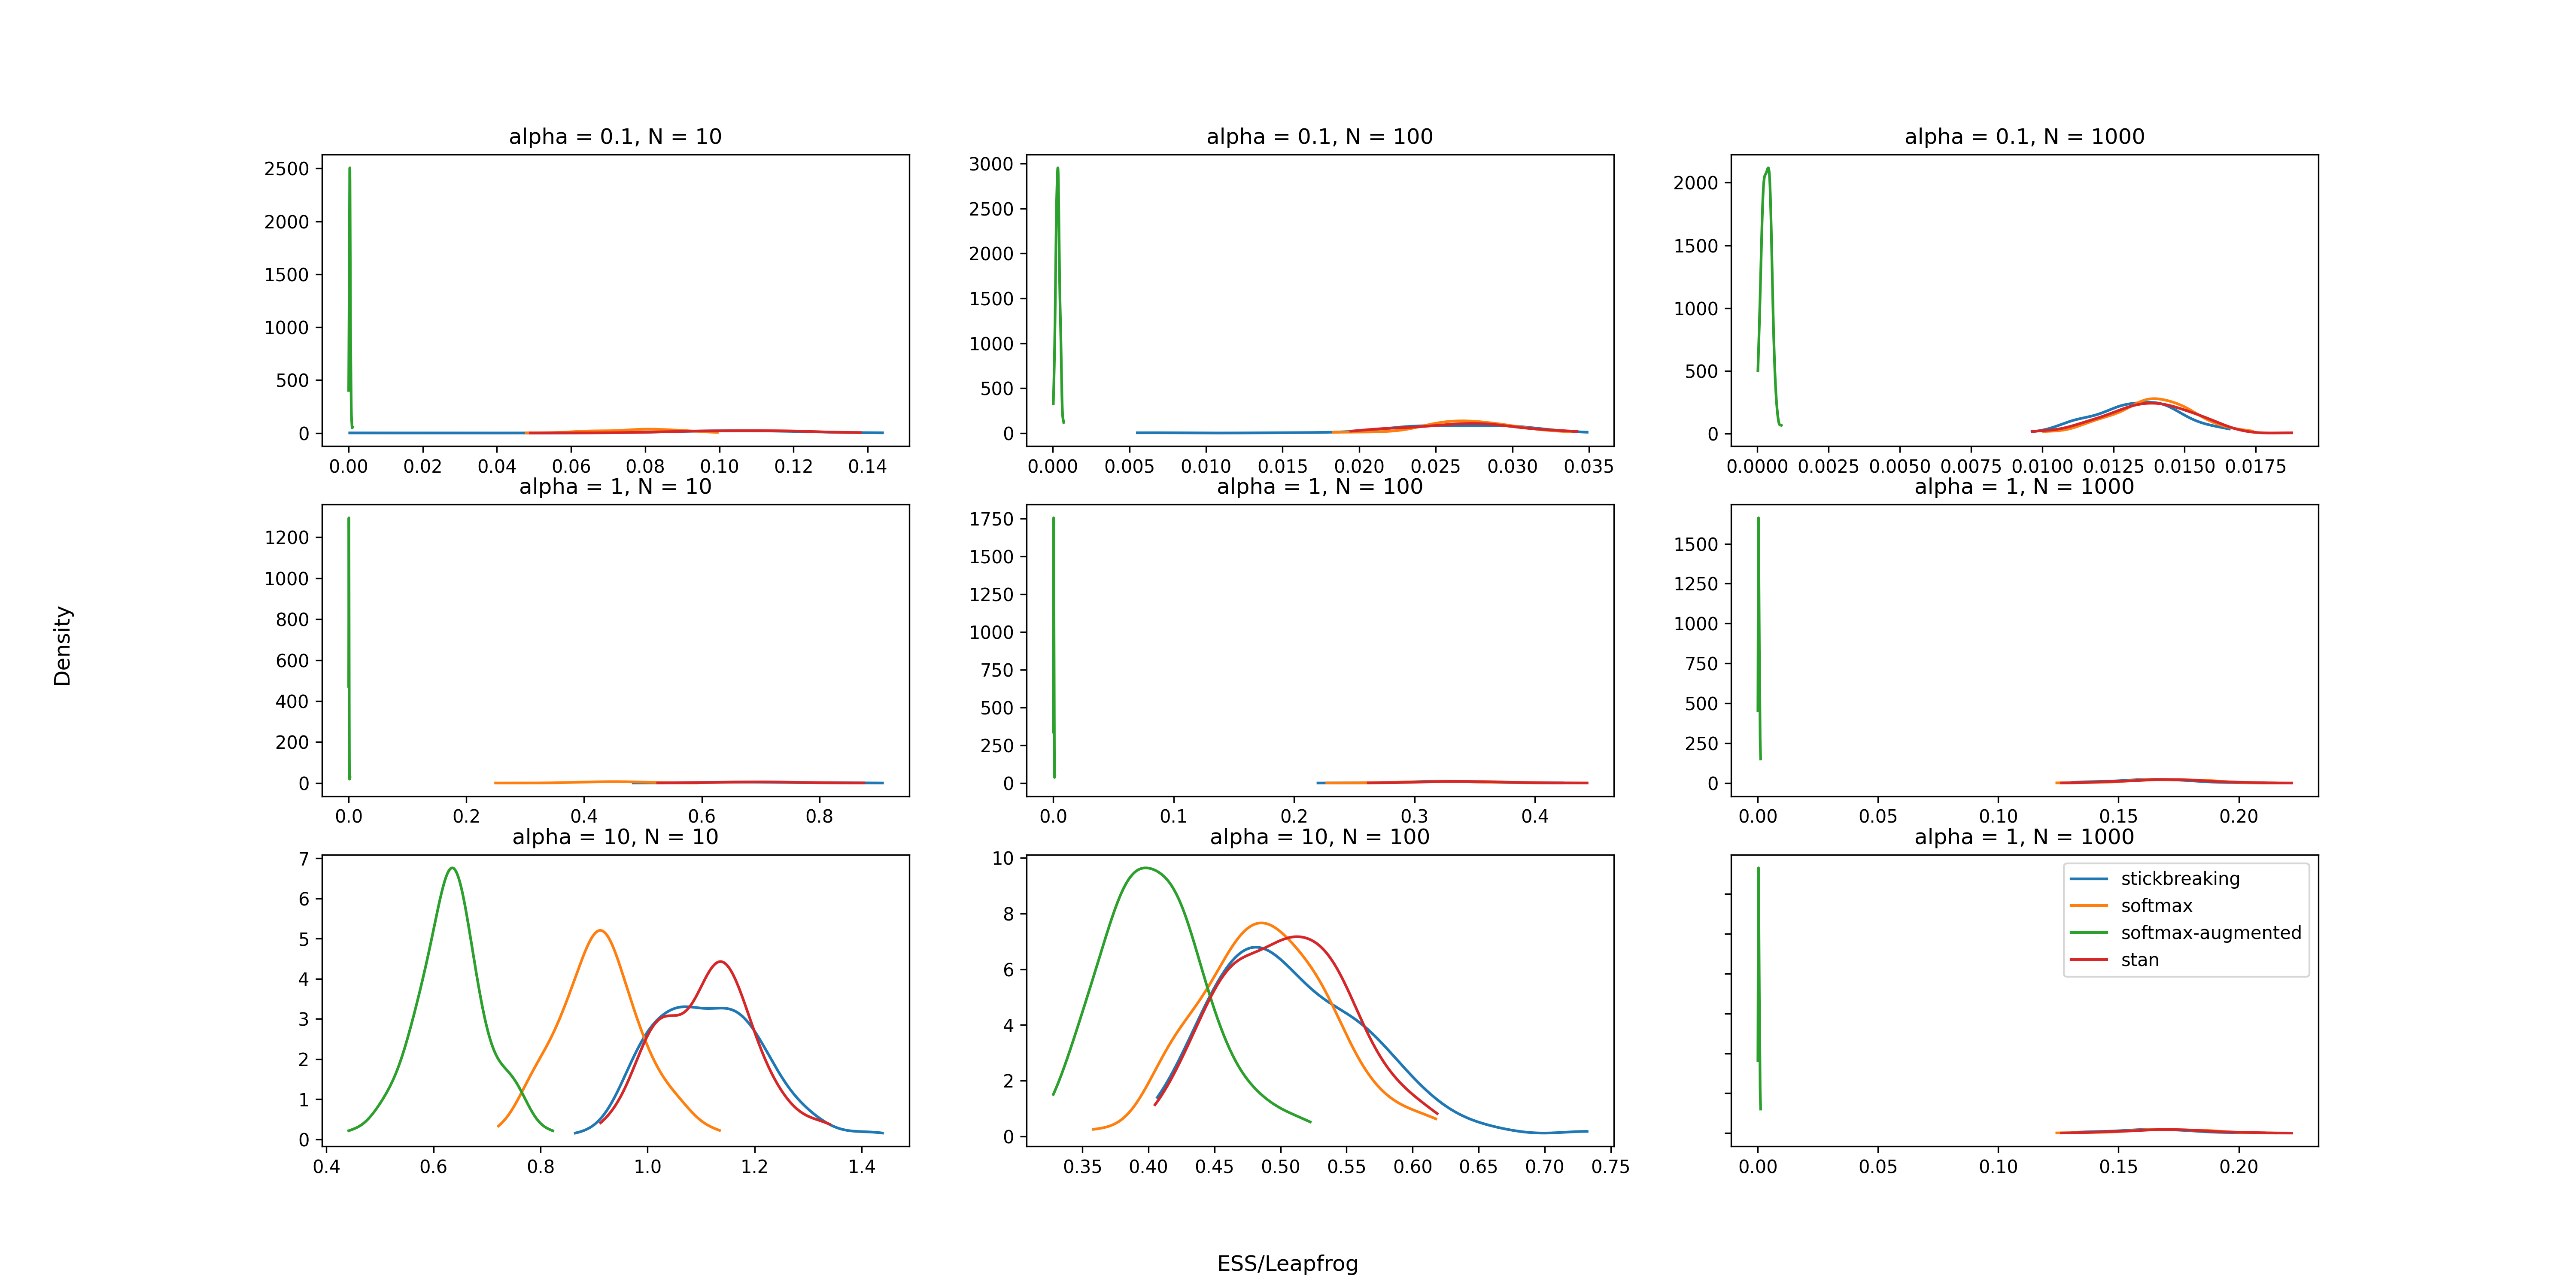
\includegraphics[width=1.2\textwidth]{figures/simplex/ess_density.png}
    \caption{Probability Density Plot of Effective Sample Size/Total Leapfrog Steps. Effective sample size is evaluated at 100 runs, and each point is the value of ESS/Total Leapfrog steps taken by the sampler in one run.}
    \label{fig:ess_density}
\end{figure}

\begin{figure}[t!]
    \centering
    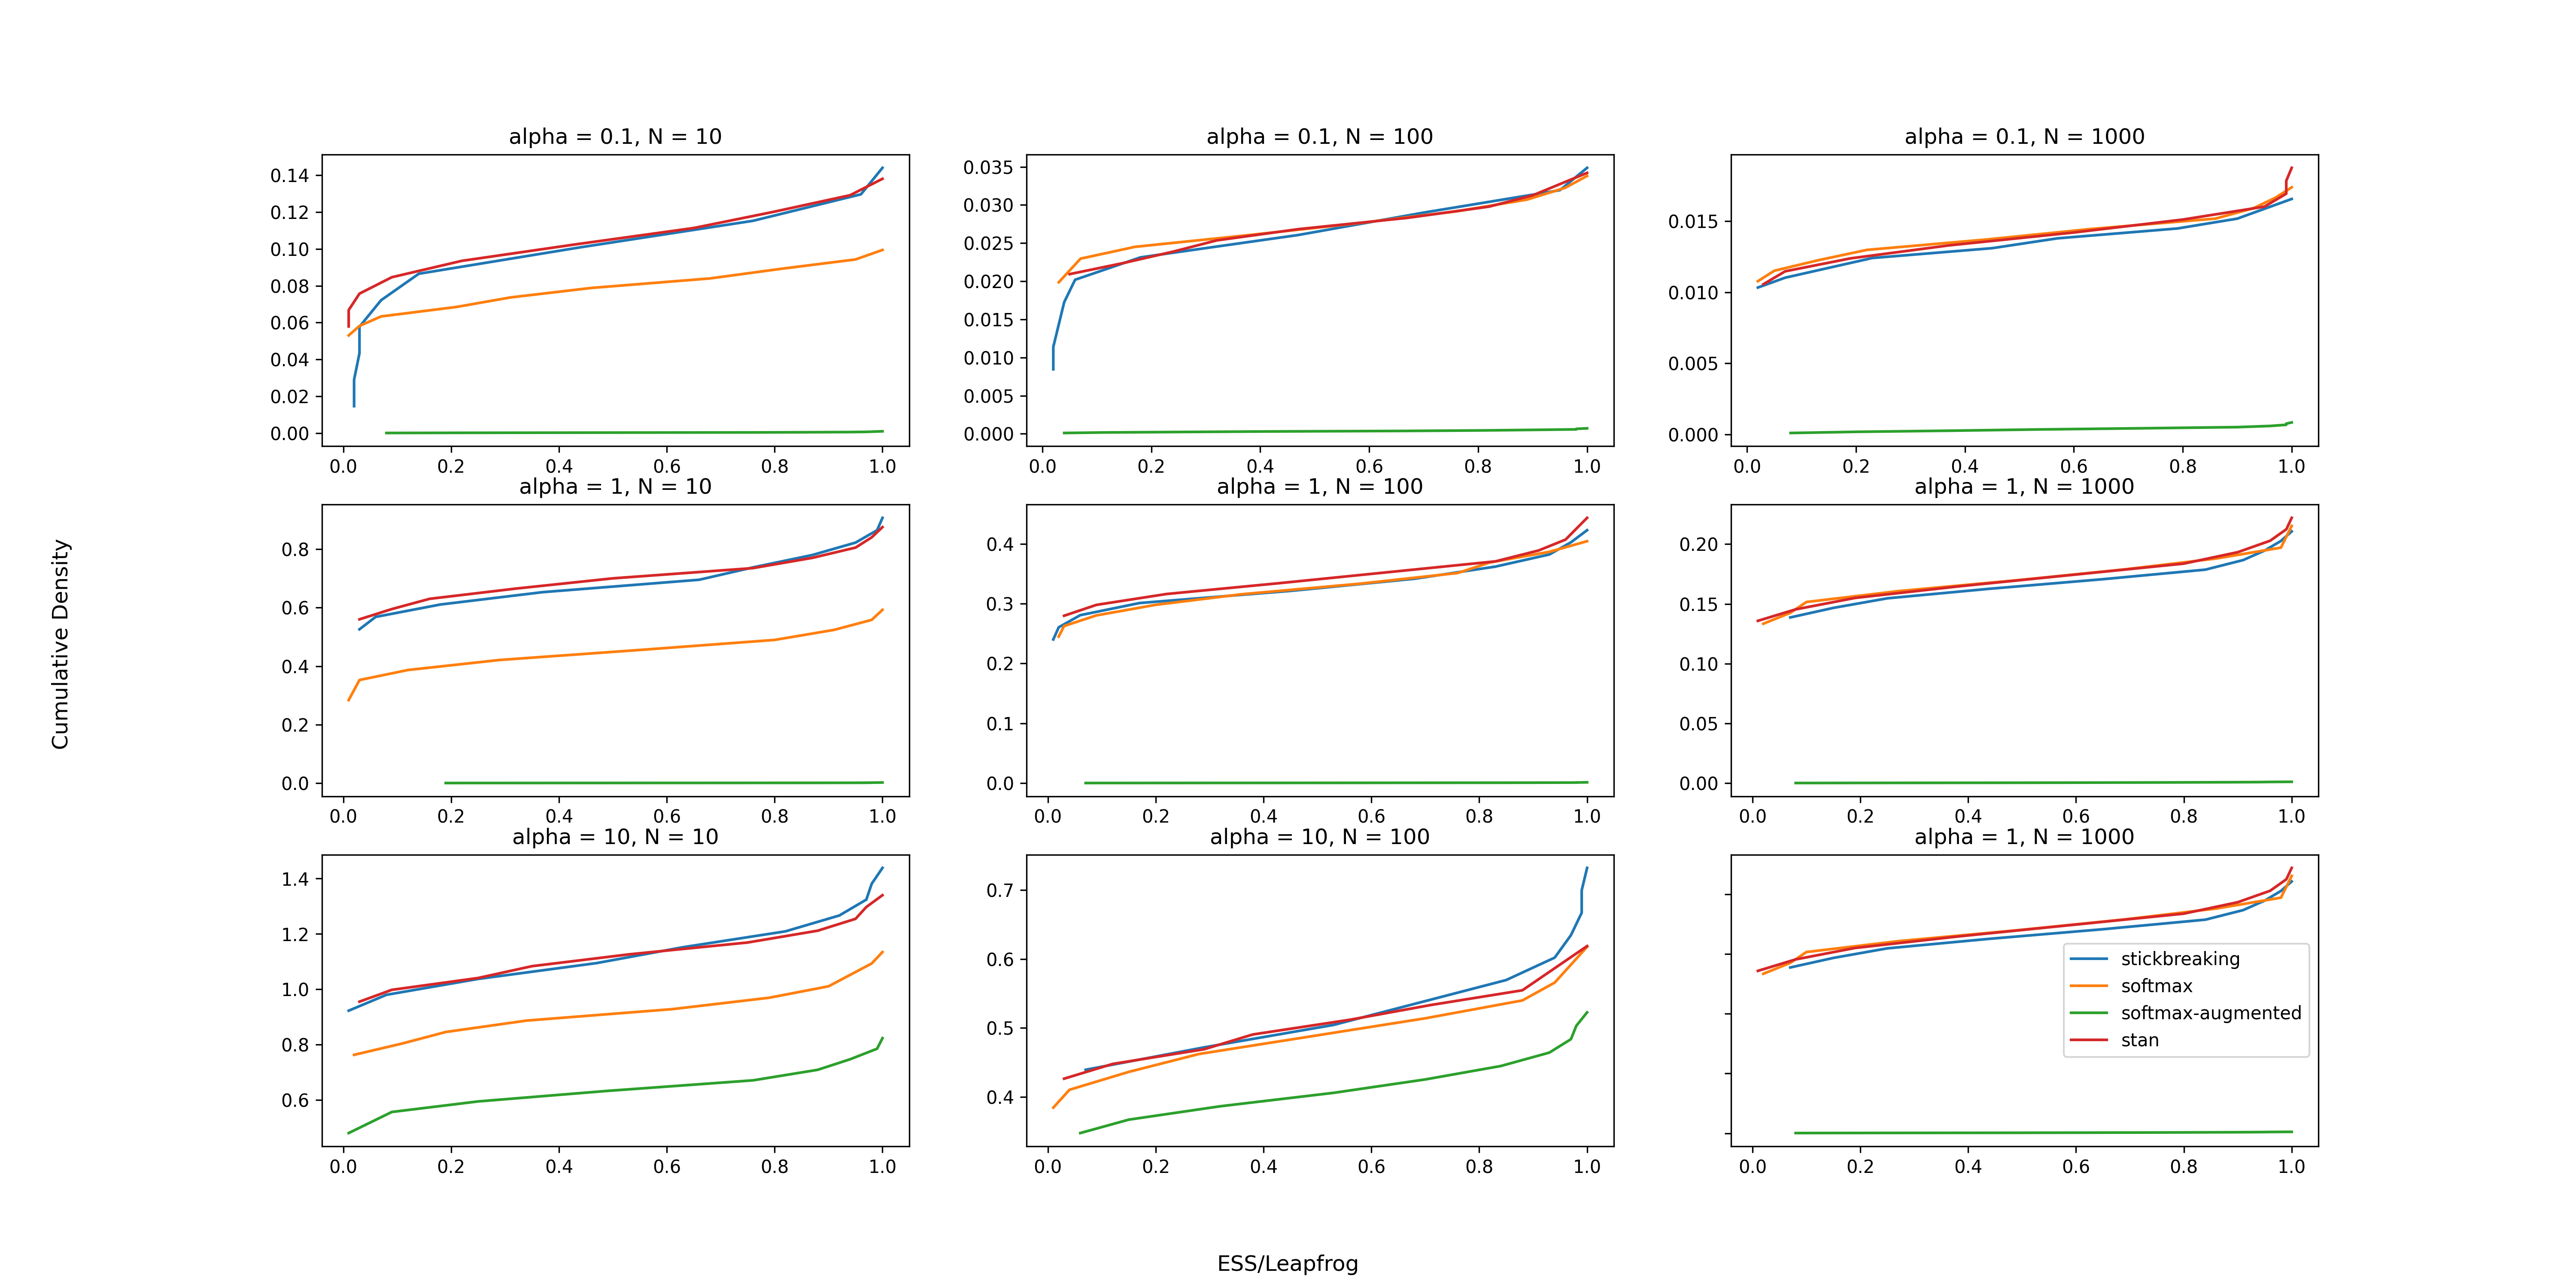
\includegraphics[width=1.2\textwidth]{figures/simplex/ess_cdf.png}
    \caption{Cumulative Density Plot of Effective Sample Size/Total Leapfrog Steps. Effective sample size is evaluated at 100 runs, each point is the value of ESS/Total Leapfrog steps taken by the sampler in one run.}
    \label{fig:ess_cdf}
\end{figure}

\begin{figure}[t!]
    \centering
    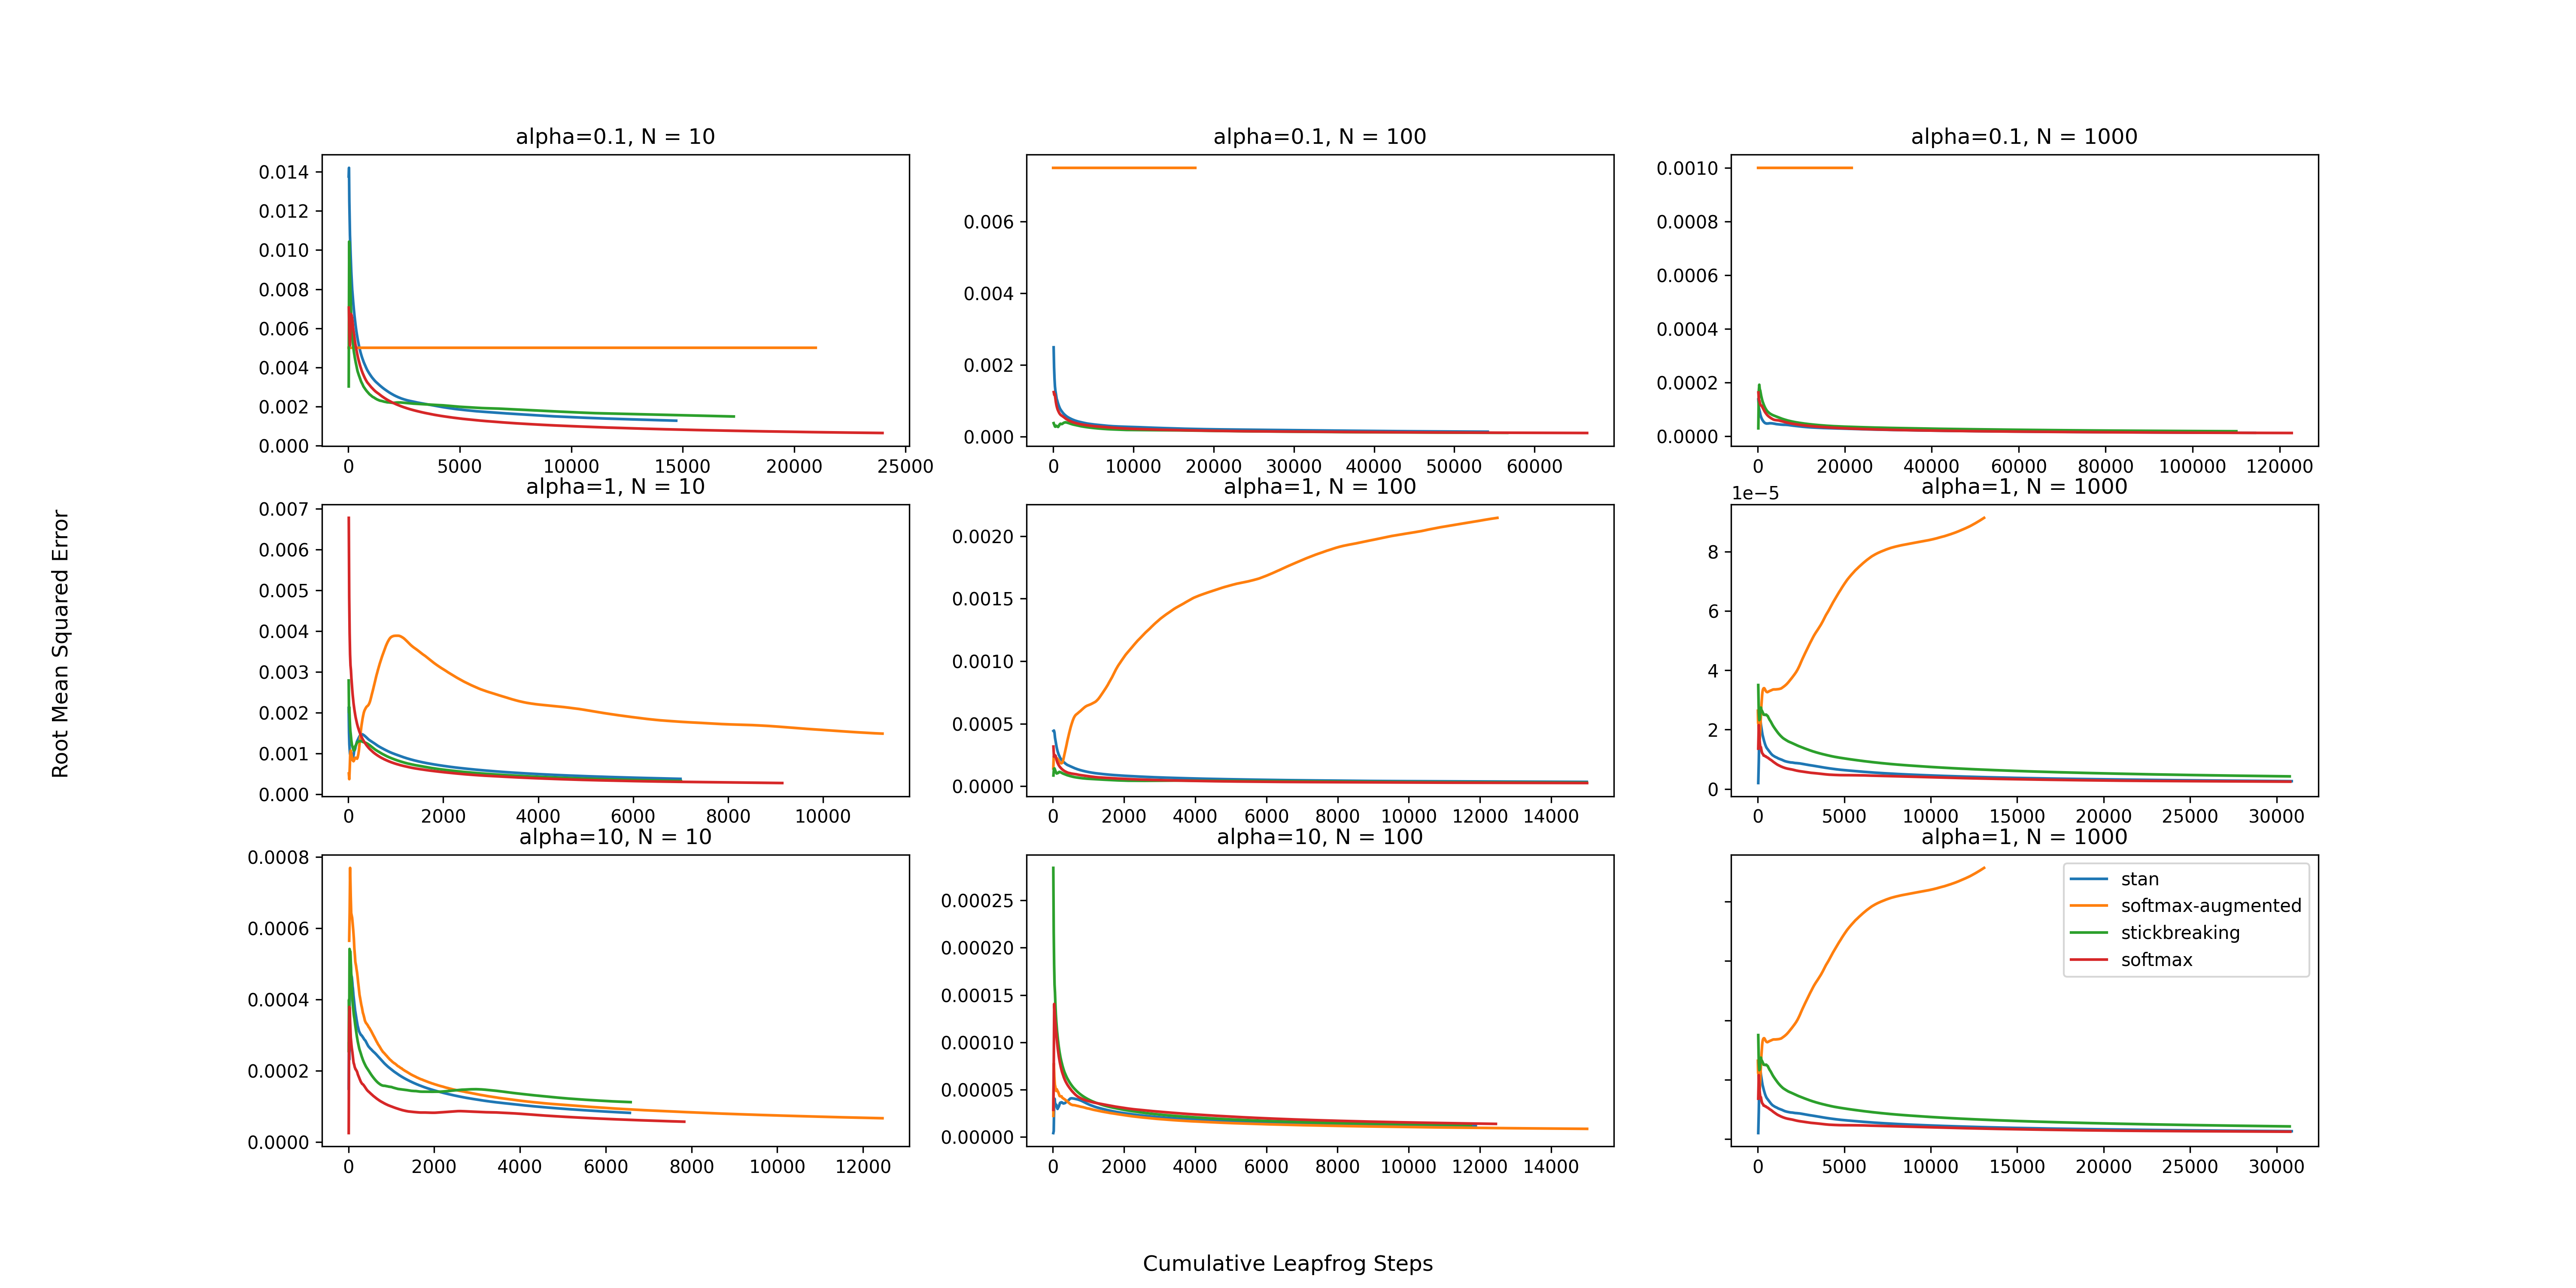
\includegraphics[width=1.2\textwidth]{figures/simplex/rmse.png}
    \caption{Root Mean Squared Error vs Cumulative Leapfrog Steps. At every iteration in a run, cumulative mean of samples is used to calculate RMSE, which is plotted against the cumulative leapfrog steps till that iteration}
    \label{fig:rmse}
\end{figure}

\subsubsection*{Acknowledgements}

We would like to thank \url{matrixcalculus.org} for providing an
easy-to-use symbolic matrix derivative calculator.
This work was funded by the Deutsche Forschungsgemeinschaft (DFG, German Research Foundation) under Germany’s Excellence Strategy – EXC number 2064/1 – Project number 390727645.


\bibliography{all}{}
\bibliographystyle{plain}

\begin{appendices}

\section{Jacobian Determinants}
\subsection{Stickbreaking Transform}
The Jacobian matrix for $f^{-1}$ is a lower-triangular diagonal matrix, so for the change of variables we evaluate $\mathbf{J}_{i, i}$ where $i \in 1:N-1$.
\begin{align*}
\mathbf{J}_{i, i} &= \frac{\partial x_i}{\partial y_i}
=
\frac{\partial x_i}{\partial z_i} \,
\frac{\partial z_i}{\partial y_i}\\
\mathbf{J}_{i, i} &= \left(
  1 - \sum_{k' = 1}^{k-1} x_{k'}
   \right) z_k (1 - z_k),\\
   \abs{\textbf{J}} &= \prod_{i=1}^{N-1} \textbf{J}_{i,i}
\end{align*}

The change of variables adjustment $p_Y(y) = p_X(f^{-1}(y))\,
\prod_{i=1}^{N-1}z_i\,(1 - z_i)\left(1 - \sum_{i'=1}^{i-1} x_{i'}\right).$

\subsection{Additive Log ratio transform}
To calculate the determinant of the Jacobian of the inverse transform,
we start by noting that $s = \textrm{exp} \circ \textrm{norm}$, where
$\textrm{exp}$ is the elementwise exponential function and
\textrm{norm} is defined by
\[
  \textrm{norm}(z) = \frac{z}{\textrm{sum}(z) + 1}.
\]
As such, the resulting Jacobian determinant is the product of the
Jacobian determinants of the component functions,
\[
  \absdet{J_s(y)}
  = \absdet{J_{\textrm{exp}}(y)} \absdet{J_{\textrm{norm}}(z)},
\]
where $z = \textrm{exp}(y)$.  The Jacobian for the exponential
function is diagonal, so the determinant is the product of the
diagonal of the Jacobian, which for $y \in \mathbb{R}^{N-1}$ is
\[
  \absdet{J_{\textrm{exp}}(y)} = \textrm{prod}(\exp(y)).
\]
As above, let $z = \exp(y) \in (0, \inf)^{N-1}$.  We can differentiate
$\textrm{norm}$ to derive the Jacobian,
\[
  J_{\textrm{norm}}
  = \frac{1}{1 + \textrm{sum}(z)} \mathbb{I}_{N-1}
  - \left(\frac{1}{(1 + \textrm{sum}(z))^2} \beta \right)
  \textrm{vector}_{N-1}(1)^{\top},
\]
where $\mathbb{I}_{N-1}$ is the $(N - 1) \times (N - 1)$ unit matrix and
$\textrm{vector}_{N-1}(1)$ is the $N - 1$-vector with values 1.  Using
the matrix determinant lemma,\footnote{The matrix determinant lemma
  is \[\textrm{det}(A + u v^{\top}) = (1 + v^{\top} A^{-1} u)
    \textrm{det}(A).\]}
we have
\begin{eqnarray*}
  \textrm{absdet}(J_{\textrm{norm}}(z))
  & = &
  \left(
    1
    + \textrm{vector}_{N-1}(1)^{\top}
    \left(\frac{1}{1 + \textrm{sum}(z)} \mathbb{I} \right)^{-1}
    \frac{-z}{(1 + \textrm{sum}(z))^2}
    \right)
    \ \textrm{det}\left(\frac{1}{1 + \textrm{sum}(z)} \mathbb{I}
        \right)
  \\[6pt]
  & = &
  \left(
    1 
    + \textrm{sum}\left( \frac{-(1 + \textrm{sum}(z)) z}{(1 +
        \textrm{sum}(z))^2} \right)
  \right)
        \ \left( \frac{1}{1 + \textrm{sum}(z)} \right)^{N-1}
  \\[6pt]
  & = &
        \left(1 + \textrm{sum}\left(\frac{-z}{1 + \textrm{sum}(z)} \right)\right)        
        \ \left( \frac{1}{1 + \textrm{sum}(z)} \right)^{N-1}
  \\[6pt]
  & = & \left( 1 - \textrm{sum}(\textrm{norm}(z)) \right) 
        \ \left( \frac{1}{1 + \textrm{sum}(z)} \right)^{N-1}
  \\[6pt]
  & = & \left( \frac{1}{1 + \textrm{sum}(z)} \right)^N.
\end{eqnarray*}
Thus the entire absolute determinant of the Jacobian is defined by the
product, 
\[
  \absdet{J_s(y)}
  \ = \
  \textrm{prod}(\exp(y))
  \, \left( \frac{1}{1 + \textrm{sum}(\exp(y))} \right)^N.
\]
and our final expression for densities for unconstrained $y \in
\mathbb{R}^{N-1}$ is
\[
  p_Y(y)
  = p_X(\textrm{alr}^{-1}(y))
  \, \textrm{prod}(\exp(y))
  \left( \frac{1}{1 + \textrm{sum}(\exp(y))} \right)^N
\]

\subsection{Hyperspherical simplex transforms}

\subsubsection{Hyperspherical coordinate transform}

We use the following definition of hyperspherical coordinates.
For $\phi_i \in (0, \pi/2]$ and $u \in \mathbb{S}^N_{>0}$, the positive orthant of the $N$-sphere,
\[
  u_i = \left(\prod_{k=1}^{i-1} \sin(\phi_k)\right) \begin{cases}
    1 & \text{ if } i = N + 1\\
    \cos(\phi_i) & \text{otherwise}
  \end{cases}.
\]

Let $z_i = \sin^2(\phi_i)$ and $x_i = u_i^2$, so that $x \in \Delta^N$.
Then
\[
  x_i = \left(\prod_{k=1}^{i-1} z_k\right) \left(\begin{cases}
    1 & \text{ if } i = N + 1\\
    (1 - z_i) & \text{otherwise}
  \end{cases}\right) = (1 - z_i (1 - \delta_{i,N+1})) \prod_{k=1}^{i-1} z_k.
\]

\subsubsection{Hyperspherical coordinates inverse transform}

To derive the inverse transform, note that
\[
    \begin{aligned}
        x_{N+1} &= \prod_{k=1}^{N} z_k\\
        x_N + x_{N+1} &= (1 - z_N)\left(\prod_{k=1}^{N-1} z_k\right) + z_N \left( \prod_{k=1}^{N-1} z_k \right) = \prod_{k=1}^{N-1} z_k = \frac{x_N}{1 - z_N}\\
        x_{N-1} + x_{N} + x_{N+1} &= (1-z_{N-1}) \left(\prod_{k=1}^{N-2} z_k\right) + z_{N-1} \left(\prod_{k=1}^{N-2} z_k\right) = \prod_{k=1}^{N-2} z_k = \frac{x_{N-1}}{1 - z_{N-1}}\\
        &\vdots \\
        \sum_{k=i}^{N+1} x_{k} &= \prod_{k=1}^{i - 1} z_k = \frac{x_i}{1 - z_i}.
    \end{aligned}
\]

From the final expression, we can define the inverse transform:
\[
z_i = 1 - \frac{x_i}{\sum_{k=i}^{N+1} x_k}
\]

\subsubsection{Jacobian of hyperspherical coordinates transform}

To derive the Jacobian, we note that $x_i$ depends only on $z_k$ for $k \le i$.
As a result, the Jacobian of the map from $z$ to $x_-$ is lower triangular, and its determinant depends only on its diagonal, which consists of the terms
$$J_{ii} = -\frac{\partial x_i}{\partial z_i} = \prod_{k=1}^{i-1} z_k,$$
so
$$
|J| = \prod_{i=1}^N |J_{ii}|
= \prod_{i=1}^N \prod_{k=1}^{i-1} z_k
= \prod_{k=1}^{N-1} \prod_{i=k+1}^N z_k
= \prod_{i=1}^{N-1} z_i^{N-i} = \prod_{i=1}^N z_i^{N-i}
$$

Due to the form of the Jacobian correction, if $x$ is uniformly distributed on the unit simplex, then $z_i$ and $z_j$ are uncorrelated for all $i \ne j$.

\subsubsection{Hyperspherical angular transform}

The map from $y$ to $z$ is elementwise, so its Jacobian is diagonal.
Each element is
$$\sin^{-1}(\sqrt{z_i}) = \phi_i = \frac{\pi}{2} \operatorname{logit}^{-1} (y_i).$$
Differentiating all sides with respect to $y_i$, we find
$$
\begin{aligned}
\frac{1}{\sqrt{1 - z_i^2}} \frac{1}{2 \sqrt{z_i}} \frac{\partial z_i}{\partial y_i} &= \frac{\pi}{2} \operatorname{logit}^{-1} (y_i) (1 - \operatorname{logit}^{-1} (y_i)) = \phi_i \left(1 - \frac{2}{\pi} \phi_i\right)\\
\frac{\partial z_i}{\partial y_i} &= 2 \phi_i \left(1 - \frac{2}{\pi} \phi_i\right) \sin(\phi_i) \cos(\phi_i).
\end{aligned}
$$

As a result, the combined transform $f: y \mapsto x$ is
\[
  x_i = \left(1 - \cos^2\left(\frac{\pi}{2} \operatorname{logit}^{-1} (y_i)\right) (1 - \delta_{i,N+1})\right)\left(\prod_{k=1}^{i-1} \sin^2\left(\frac{\pi}{2} \operatorname{logit}^{-1} (y_k)\right)\right),
\]
and its inverse is
\[
z_i = \operatorname{logit}\left(\frac{2}{\pi}\sin^{-1}\left(\sqrt{1 - \frac{x_i}{\sum_{k=i}^{N+1} x_k}}\right)\right).
\]

The Jacobian determinant is
$$
\begin{aligned}
    |J_f| &= \prod_{i=1}^N z_i^{N-i} 2 \phi_i \left(1 - \frac{2}{\pi} \phi_i\right) \sin(\phi_i) \cos(\phi_i)\\
          &= 2^N \prod_{i=1}^N \phi_i \left(1 - \frac{2}{\pi} \phi_i\right) \sin^{2(N-i)+1}(\phi_i) \cos(\phi_i).
\end{aligned}
$$

\subsubsection{Hyperspherical logit transform}

For $z_i \in (0, 1]$, $z_i^k \in (0, 1]$ is bijective for $k \ne 0$.
Let $g(w)$ be the density function for a distribution on $\mathbb{R}$ and $G(w)$ be its cumulative distribution function.
By the definition of the CDF, $\frac{\mathrm{d}}{\mathrm{d}w} G(w) = g(w)$.
Let $z_i^{N-i+1} = G(y_i)$.

The combined transform $f: y \mapsto x$ is then
\[
  x_i = \left(1-G(y_i)^{1/(N-i+1)}(1 - \delta_{i,N+1})\right)\left(\prod_{k=1}^{i-1} G(y_k)^{1/(N-k+1)}\right),
\]
and its inverse is 
\[
y_i = G^{-1}\left(\left(1 - \frac{x_i}{\sum_{k=i}^{N+1} x_k}\right)^{N-i+1}\right).
\]

Then
$$
\begin{aligned}
(N-i+1) z_i^{N-i} \frac{\partial z_i}{\partial y_i} &= g(y_i)\\
\frac{\partial z_i}{\partial y_i} &= \frac{g(y_i)}{(N-i+1) z_i}.
\end{aligned}
$$

As a result,
$$
\begin{aligned}
|J_f| &= \prod_{i=1}^{N} z_i^{N-i} \frac{g(y_i)}{(N-i+1) z_i^{N-i}}\\ 
&= \left(\prod_{i=1}^N \frac{1}{N-i+1} \right) \prod_{i=1}^{N} g(y_i)\\
&= \frac{1}{N!} \prod_{i=1}^{N} g(y_i).
\end{aligned}
$$

This particular transform allows us to transform the uniform distribution on the simplex to any distribution on $\mathbb{R}^N$ whose coordinates are IID distributed according to $g$.

If we select $G$ to be the logistic function, then $g(w) = \operatorname{logit}^{-1}(w) (1 - \operatorname{logit}^{-1}(w))$ is the density of the logistic distribution with mean $0$ and scale term $1$, and $y_i$ is logistically distributed.
This choice of $G$ defines the hyperspherical logit transform.

\subsubsection{Hyperspherical probit transform}

Similarly, to define the hyperspherical probit transform, we select $G$ to be the inverse probit function.
Then $g$ is the density function of the standard normal distribution.

\subsubsection{Transforming the Dirichlet distribution}

Recall that the Dirichlet distribution has density $p_X(x)$ equal to
\[
p_X(x) \propto \prod_{i=1}^{N+1} x_i^{\alpha_i - 1}.
\]

Note that
\[
\begin{aligned}
\prod_{i=1}^{N+1} x_i^{\alpha_i - 1} &= \prod_{i=1}^{N+1} \left(\left(1-G(y_i)^{1/(N-i+1)}(1 - \delta_{i,N+1})\right)\left(\prod_{k=1}^{i-1} G(y_k)^{1/(N-k+1)}\right)\right)^{\alpha_i - 1}\\
&= \left(\prod_{i=1}^{N} \left(1-G(y_i)^{1/(N-i+1)}\right)^{\alpha_i - 1}\right) \prod_{i=1}^{N+1}\prod_{k=1}^{i-1} G(y_k)^{(\alpha_i - 1)/(N-k+1)}\\
&= \prod_{i=1}^{N} \left(1-G(y_i)^{1/(N-i+1)}\right)^{\alpha_i - 1} G(y_i)^{-1+\sum_{k=i+1}^{N+1}\alpha_k/(N-i+1)}\\
\end{aligned}
\]
The transformed density on $y$ is then
\[
p_Y(y) \propto \prod_{i=1}^{N} \left(1-G(y_i)^{1/(N-i+1)}\right)^{\alpha_i - 1} G(y_i)^{-1+\sum_{k=i+1}^{N+1}\alpha_k/(N-i+1)} g(y_i) = \prod_{i=1}^{N} h(y_i, \alpha_{i:N+1}),
\]
where $h$ is a density function.
Therefore, regardless of the choice of $g$ or $\alpha$, the individual coordinates of the transformed distribution are independently distributed.
\end{appendices}
\end{document}
